\chapter{Problem Analysis}\label{ch:problemAnalysis}
\section{Problem Description}
Humans have the ability to identify the source of a sound around them. In the 
field of neuroscience, this capability is called sound localization. The brain
can determine the location of a sound with very high precision, up to 2 degrees 
of space. This comes from the brain's capacity to interpret information received
from both ears.\cite{HUMANSOUNDS2}

Over the years, neuroscientists, have been trying to understand the mechanisms 
within our brains that are able to determine the location of a sound. They have 
identified two cues that are essential and sufficient for horizontal sound
localization.

In the 1790s, Giovanni Battista Venturi conducted experiments where he played a 
flute around blindfolded people and asked them to point in his direction. 
He concluded that the sound amplitude difference between the two ears was the 
indicator used for determining the direction.

Much later, Malloch proposed that the difference in time between the two ears 
was the sign used for determining the direction of a sound.

Years later, scientists found neurons in the auditory center of the brain
specially adjusted for each indicator: time and intensity differences between 
the two ears.\cite{HUMANSOUNDS}

\newpage

Figure \ref{fig:humanHearingAccuracy} shows a circle, and a person in the middle. 
The person is meant to be the listener, while the circle represents a perfectly 
flat plane around the listeners head.
 
\begin{figure}[htp]
	\centering
	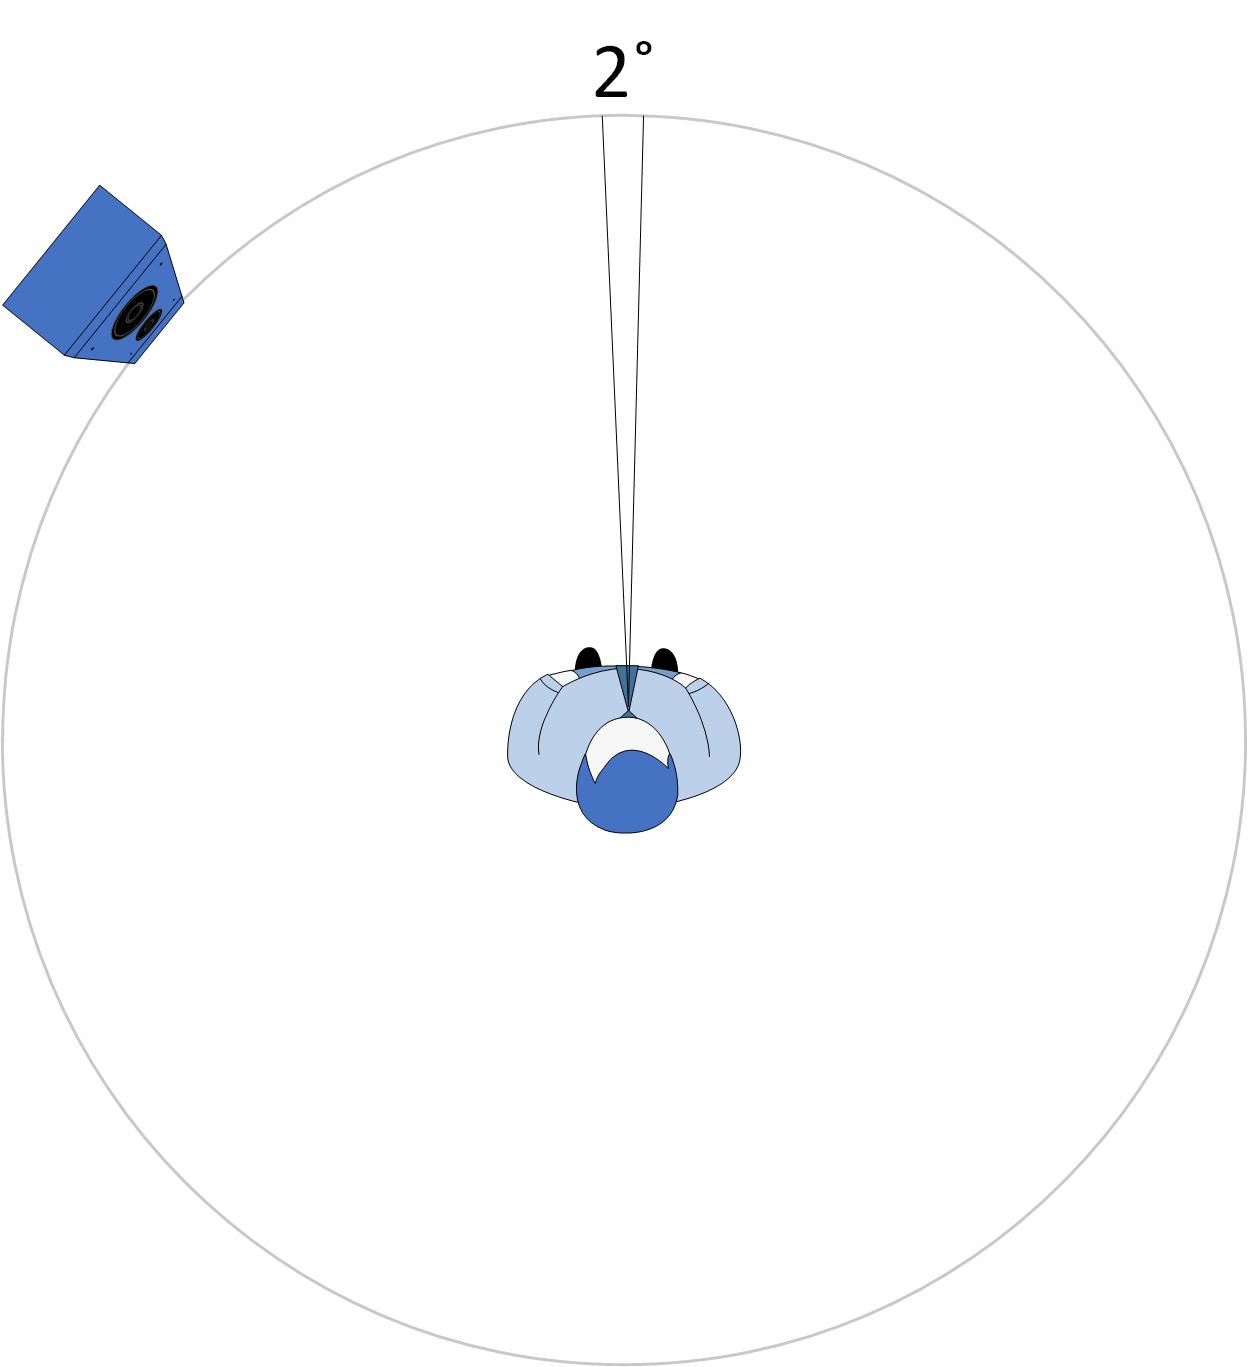
\includegraphics[width = 0.6\textwidth]{Illustrations/personHearingAccuracy.jpg}
	\caption{Human Hearing Accuracy}
	\label{fig:humanHearingAccuracy}
\end{figure}

Sound coming from the speaker, would reach  the right year faster and be louder than 
the sound that reaches the left year. The brain is able to compare the differences
and tell where the sound is coming from.

Human voice frequency ranges from male to female. A female voice frequency ranges from 
350Hz to 17KHz, while a male's ranges from 100Hz to 8Khz. This needs to be taken into
account when recording. Making sure the sampling frequency is high enough to avoid 
aliasing of the signal is crucial.\cite{VOICEFREQUENCY}
\newpage
\section{Problem Delimitation}
This report focuses on the research of different methods of filtering. We did not
look in depth into how this research could be useful to real world applications. Instead we 
focused on our own studying and trying to learn as much out of it as possible.
\todo[inline]{maybe write some more shit}
\section{Tools}
The following list contains tools and softwares used for the development of the filters:
\begin{itemize}
\item Python 3.6
\item Anaconda 1.7.2
\item Jupyter Notebook
\item TensorFlow 1.13
\item Keras 2.2.4
\item cuDNN 8.0
\item CUDA 9.0
\item Matlab R2018a
\item Microsoft Visio 2016
\item Adobe Audition CC 2018
\end{itemize}